% This file was created with tikzplotlib v0.10.1.
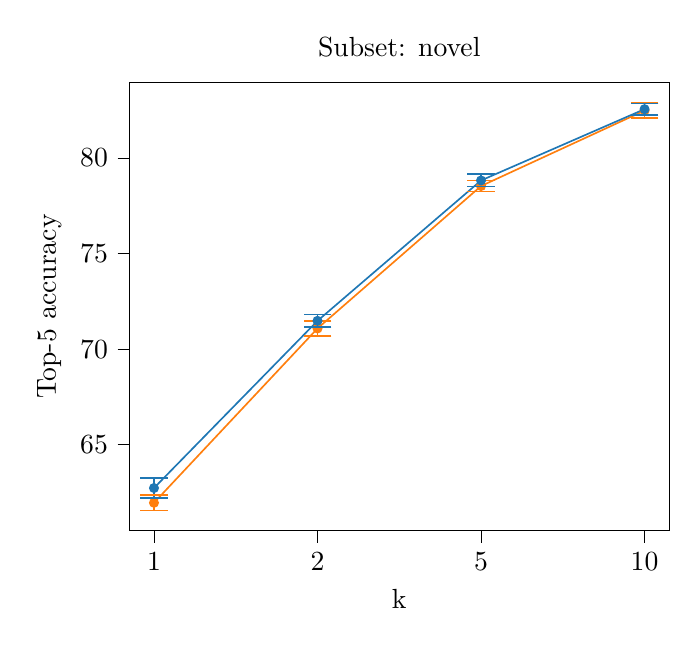
\begin{tikzpicture}

\definecolor{darkgray176}{RGB}{176,176,176}
\definecolor{darkorange25512714}{RGB}{255,127,14}
\definecolor{lightgray204}{RGB}{204,204,204}
\definecolor{steelblue31119180}{RGB}{31,119,180}

\begin{axis}[
legend cell align={left},
legend style={
  fill opacity=0.8,
  draw opacity=1,
  text opacity=1,
  at={(0.97,0.03)},
  anchor=south east,
  draw=lightgray204
},
tick align=outside,
tick pos=left,
title={Subset: novel},
x grid style={darkgray176},
xlabel={k},
xmin=-0.15, xmax=3.15,
xtick style={color=black},
xtick={0,1,2,3},
xtick={0,1,2,3},
xtick={0,1,2,3},
xtick={0,1,2,3},
xtick={0,1,2,3},
xtick={0,1,2,3},
xticklabels={1,2,5,10},
xticklabels={1,2,5,10},
xticklabels={1,2,5,10},
xticklabels={1,2,5,10},
xticklabels={1,2,5,10},
xticklabels={1,2,5,10},
y grid style={darkgray176},
ylabel={Top-5 accuracy},
ymin=60.4949736662386, ymax=83.9517212149162,
ytick style={color=black}
]

\path [draw=darkorange25512714, semithick]
(axis cs:0,61.5611894639058)
--(axis cs:0,62.3616401180878);

\path [draw=darkorange25512714, semithick]
(axis cs:1,70.6993290183528)
--(axis cs:1,71.4665873803611);

\path [draw=darkorange25512714, semithick]
(axis cs:2,78.2504533010468)
--(axis cs:2,78.8170708147088);

\path [draw=darkorange25512714, semithick]
(axis cs:3,82.0791248078314)
--(axis cs:3,82.885505417249);

\path [draw=steelblue31119180, semithick]
(axis cs:0,62.1986523071615)
--(axis cs:0,63.2675856349607);

\path [draw=steelblue31119180, semithick]
(axis cs:1,71.1533675453303)
--(axis cs:1,71.8099765061167);

\path [draw=steelblue31119180, semithick]
(axis cs:2,78.502138954217)
--(axis cs:2,79.1493079911206);

\path [draw=steelblue31119180, semithick]
(axis cs:3,82.2532127531485)
--(axis cs:3,82.8606136134109);


\addplot [semithick, darkorange25512714, mark=-, mark size=5, mark options={solid}, only marks]
table {%
0 61.5611894639058
1 70.6993290183528
2 78.2504533010468
3 82.0791248078314
};
% \addlegendentry{KGTN (baseline)}
\addplot [semithick, darkorange25512714, mark=-, mark size=5, mark options={solid}, only marks]
table {%
0 62.3616401180878
1 71.4665873803611
2 78.8170708147088
3 82.885505417249
};
% \addlegendentry{KGTN (baseline)}
\addplot [semithick, darkorange25512714, mark=*, mark size=1.5, mark options={solid}]
table {%
0 61.9614147909968
1 71.0829581993569
2 78.5337620578778
3 82.4823151125402
};
% \addlegendentry{KGTN (baseline)}
\addplot [semithick, steelblue31119180, mark=-, mark size=5, mark options={solid}, only marks]
table {%
0 62.1986523071615
1 71.1533675453303
2 78.502138954217
3 82.2532127531485
};
% \addlegendentry{KGTN (baseline)}
\addplot [semithick, steelblue31119180, mark=-, mark size=5, mark options={solid}, only marks]
table {%
0 63.2675856349607
1 71.8099765061167
2 79.1493079911206
3 82.8606136134109
};
% \addlegendentry{KGTN (baseline)}
\addplot [semithick, steelblue31119180, mark=*, mark size=1.5, mark options={solid}]
table {%
0 62.7331189710611
1 71.4816720257235
2 78.8257234726688
3 82.5569131832797
};
% \addlegendentry{KGTN-ens (ours)}
\end{axis}

\end{tikzpicture}
